\documentclass[border=4pt]{standalone}

\usepackage{amsmath}
\usepackage{tikz}
\usepackage{mathdots}
\usepackage{yhmath}
\usepackage{cancel}
\usepackage{color}
\usepackage{siunitx}
\usepackage{array}
\usepackage{multirow}
\usepackage{amssymb}
\usepackage{gensymb}
\usepackage{tabularx}
\usepackage{booktabs}
\usetikzlibrary{fadings}
\usetikzlibrary{patterns}


\begin{document}
 
\tikzset{every picture/.style={line width=0.75pt}} %set default line width to 0.75pt

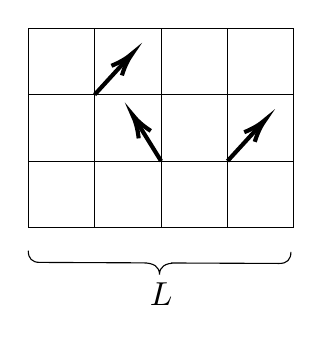
\begin{tikzpicture}[x=0.75pt,y=0.75pt,yscale=-0.8,xscale=0.8]
%uncomment if require: \path (0,300); %set diagram left start at 0, and has height of 300

%Shape: Grid [id:dp25208931655405464]
\draw  [draw opacity=0] (191,85) -- (351,85) -- (351,205) -- (191,205) -- cycle ; \draw   (231,85) -- (231,205)(271,85) -- (271,205)(311,85) -- (311,205) ; \draw   (191,125) -- (351,125)(191,165) -- (351,165) ; \draw   (191,85) -- (351,85) -- (351,205) -- (191,205) -- cycle ;
%Straight Lines [id:da5962653576884264]
\draw [line width=1.5]    (231,125) -- (251.81,102.24) ;
\draw [shift={(253.83,100.03)}, rotate = 492.44] [color={rgb, 255:red, 0; green, 0; blue, 0 }  ][line width=1.5]    (14.21,-4.28) .. controls (9.04,-1.82) and (4.3,-0.39) .. (0,0) .. controls (4.3,0.39) and (9.04,1.82) .. (14.21,4.28)   ;

%Straight Lines [id:da1028407094136734]
\draw [line width=1.5]    (311,165) -- (331.81,142.24) ;
\draw [shift={(333.83,140.03)}, rotate = 492.44] [color={rgb, 255:red, 0; green, 0; blue, 0 }  ][line width=1.5]    (14.21,-4.28) .. controls (9.04,-1.82) and (4.3,-0.39) .. (0,0) .. controls (4.3,0.39) and (9.04,1.82) .. (14.21,4.28)   ;

%Straight Lines [id:da1171571691861637]
\draw [line width=1.5]    (271,165) -- (255.24,139.55) ;
\draw [shift={(253.66,137)}, rotate = 418.23] [color={rgb, 255:red, 0; green, 0; blue, 0 }  ][line width=1.5]    (14.21,-4.28) .. controls (9.04,-1.82) and (4.3,-0.39) .. (0,0) .. controls (4.3,0.39) and (9.04,1.82) .. (14.21,4.28)   ;

%Shape: Brace [id:dp6670021980689129]
\draw   (191,219) .. controls (190.98,223.67) and (193.3,226.01) .. (197.97,226.03) -- (260.06,226.3) .. controls (266.73,226.33) and (270.05,228.68) .. (270.03,233.34) .. controls (270.05,228.68) and (273.39,226.36) .. (280.06,226.39)(277.06,226.38) -- (342.15,226.66) .. controls (346.82,226.68) and (349.16,224.36) .. (349.18,219.69) ;

% Text Node
\draw (271,245) node [scale=1.2]  {$L$};


\end{tikzpicture}



\end{document}
